\section{Resonance Search in the dijet mass spectrum}
\label{sec:background}



The resolution for the $m_\mathrm{jj}$ reconstruction is 
in the range $5 - 10\% $ for all the five categories.
The background from multijet events is modelled by a smoothly falling
distribution for each event category, given by the empirical
probability density function
\begin{equation}
P_D(m_\mathrm{jj}) = \frac{P_{0} (1 - m_\mathrm{jj}/\sqrt{s})^{P_{1}}}{(m_\mathrm{jj}/\sqrt{s})^{P_{2}}} \ .
\label{eqParam}
\end{equation}
\noindent 
%For each category, the normalization factor $P_0$ and the
%two shape parameters $P_1$ and $P_2$ are treated 
%as uncorrelated. 
Each event category has separate normalization $P_0$ and shape parameters $P_1$
and $P_2$.
This
parameterization was deployed successfully in a number of 
searches based on dijet mass
spectra~\cite{cmsdijet}. A Fisher F-test~\cite{Ftest} is used to check
that no additional parameters are needed to model the individual
background distributions, compared with the four-parameter function used in~\cite{cmsdijet}.
%We have also tested an alternative function $P_E(m_\mathrm{jj}) = \frac{P_{0}}{{(m_\mathrm{jj}/\sqrt{s} + P_{1})}^{P_{2}}}$,
We have also tested an alternative function $P_E(m_\mathrm{jj}) = P_{0}/{(m_\mathrm{jj}/\sqrt{s} + P_{1})}^{P_{2}}$,
and found it less favored by the F-test.
%The changes in the result are negligible so no additional systematic uncertainty
%is assigned for this.
The use of the alternative function in 
the analysis produces negligible changes
in the final result and therefore, no systematic 
uncertainty is associated with
this choice.

We search for a peak on top of the falling background spectrum by
means of a binned maximum likelihood fit to the data. 
%The events are binned as a function of $m_\mathrm{jj}$ with the 
%bin width of 1~\GeV.  Such narrow bin width is significantly smaller 
%than the bin width used to display data, which is proportional to the
%resolution on $m_\mathrm{jj}$.
The binned likelihood is given by
\begin{equation} \mathcal{L} = \prod_{i}
  %\frac{\lambda_{i}^{n_{i}}\re^{-\lambda_{i}}}{n_{i}!},
  \frac{\lambda_{i}^{n_{i}} e^{-\lambda_{i}}}{n_{i}!},
\end{equation}
where ${\lambda_{i}} = {\mu}{N_{i}(S)} + {N_{i}(B)}$,
$\mu$ is a scale factor for the signal, $N_i(S)$ is the number
of events expected from the signal, 
and $N_i(B)$ is the number expected from
multijet background. The variable 
$n_i$ quantifies the number of observed
events in the $i^\mathrm{th}$ $m_\mathrm{jj}$ bin.
The number of background events 
$N_i(B)$ is described by the functional form of
Eq.~(\ref{eqParam}). 
While maximizing the likelihood, 
$\mu$ as well as the parameters of the background
function are unconstrained and left floating.
For presentational purposes, a binning according to $m_\mathrm{jj}$ resolution 
is used in this paper.  However, the likelihood is calculated
in bins of 1 GeV in $m_\mathrm{jj}$, 
approximating an unbinned analysis,
while keeping it computationally manageable.

Figures~\ref{fig:HbbZqqBG} and~\ref{fig:HwwZqqBG} 
show the $m_\mathrm{jj}$ distributions in data, binned according to
$m_\mathrm{jj}$ resolution.   
The solid
curves represent the results of the maximum likelihood fit to the data,
fixing the number of expected signal events to zero, while the bottom
panels show the corresponding pull distributions, quantifying the
agreement between the background-only hypothesis and the data.
The expected distributions of \HbbVqq~and \HwwVqq~signals at 
1.0, 1.5 and 2.0 \TeVcc in each category, 
scaled to their corresponding cross sections  
are given by the dashed and dash-dotted
curves.
The resonance masses in \HbbAll\ channels are slightly lower than 
those of the \HWWAll\ channels because of missing
neutrinos in b-hadron decays
and partial misreconstruction of two-pronged ${\rm\Hbb}$ decays. 



\begin{figure}[th!b]
\begin{center}
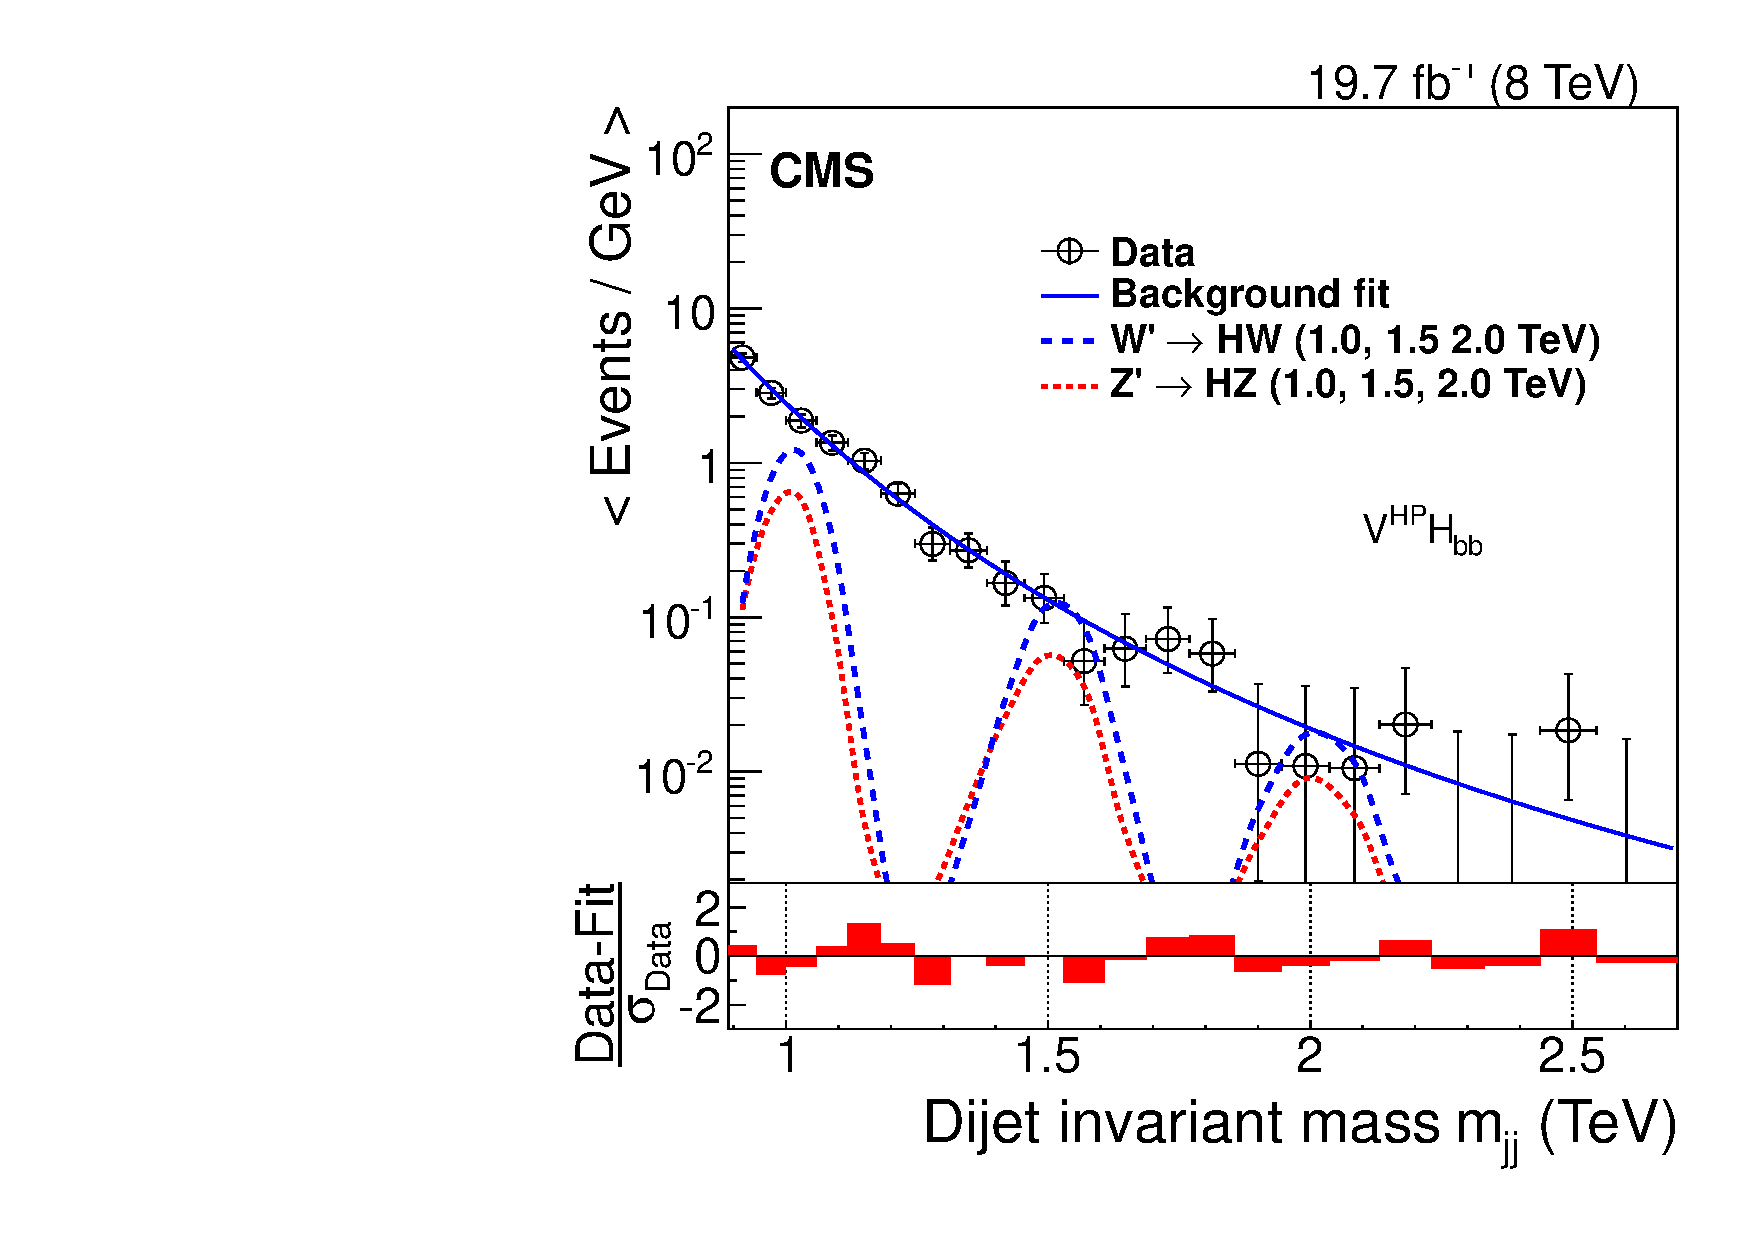
\includegraphics[width=0.49\textwidth]{EXO-14-009/HbbZqqfigs/FITS/HbbVqqFitAndPullHighP.pdf}
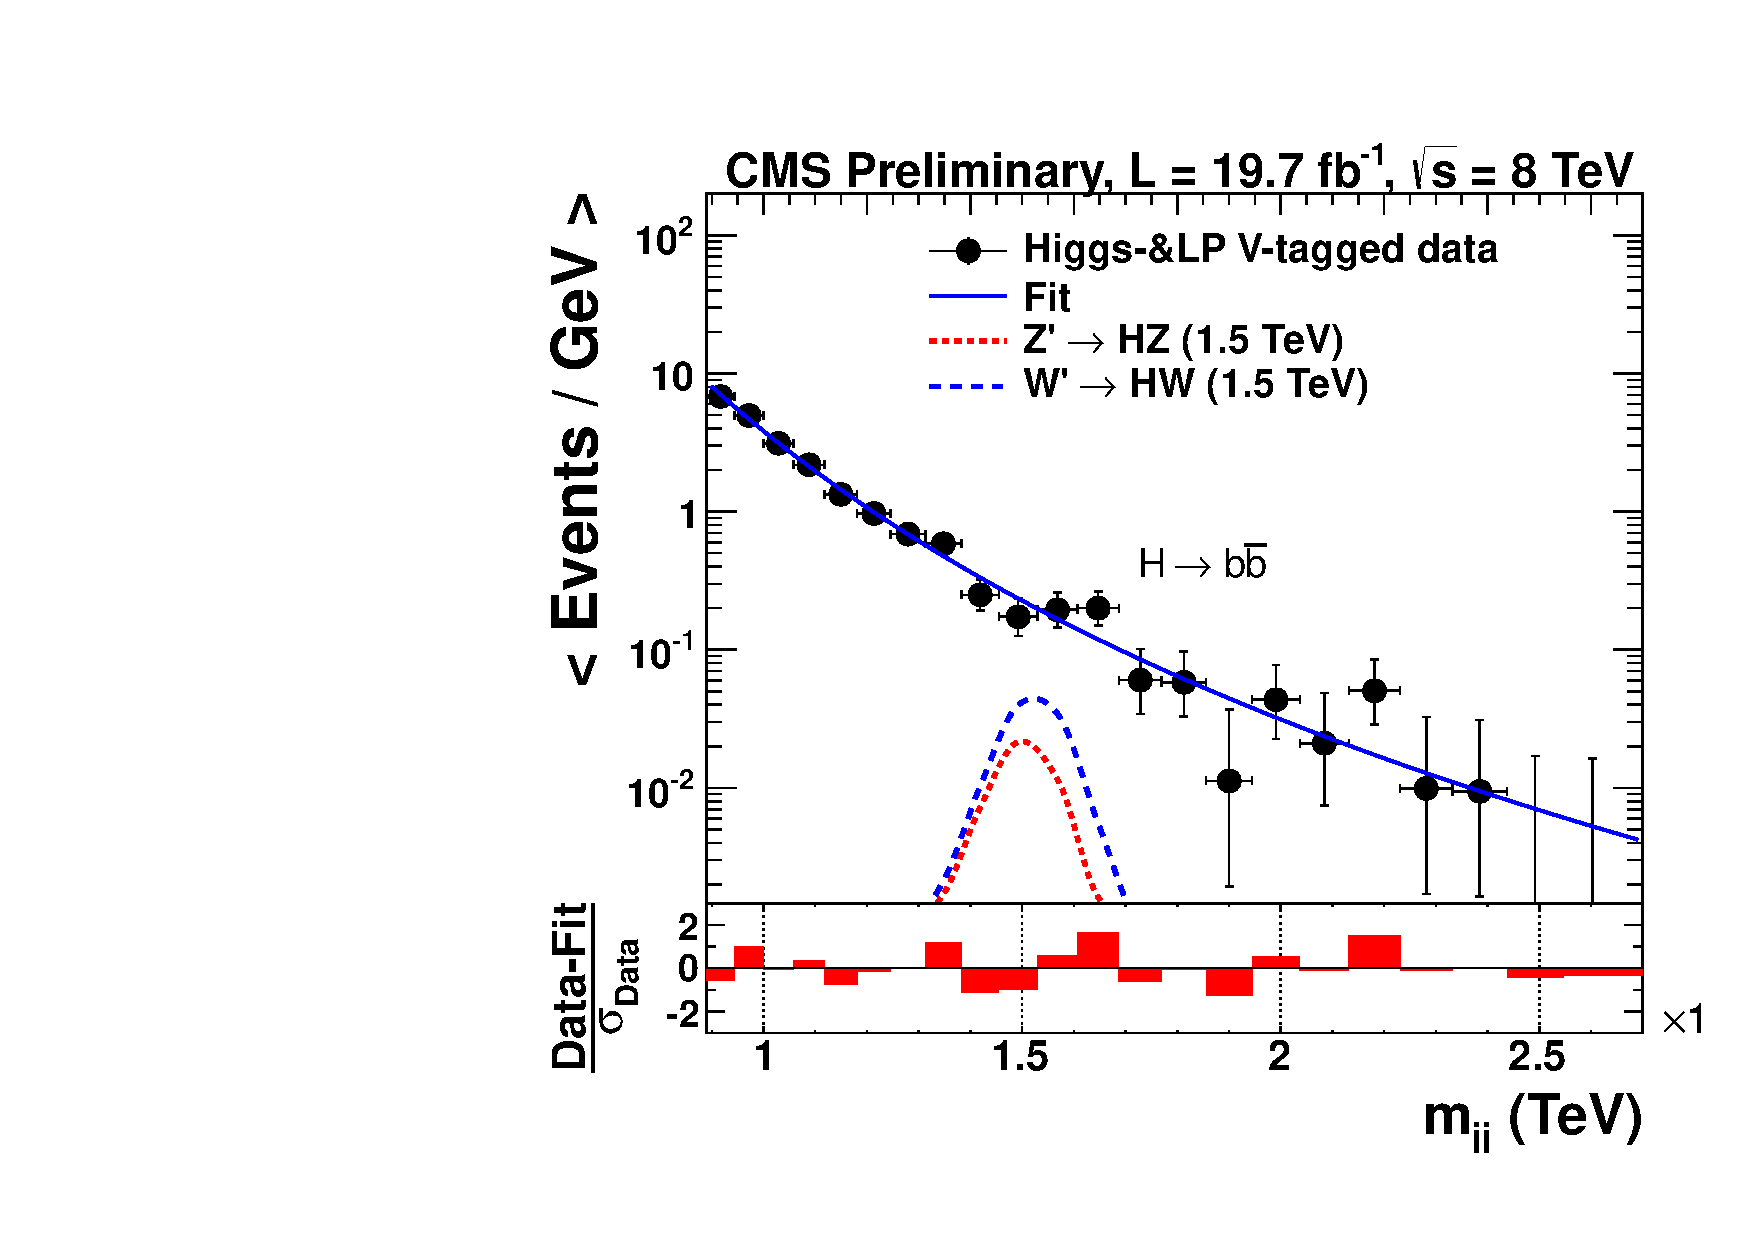
\includegraphics[width=0.49\textwidth]{EXO-14-009/HbbZqqfigs/FITS/HbbVqqFitAndPullLowP.pdf}
\end{center}
\caption{Distributions in $m_\mathrm{jj}$ are shown for
   \HbbHP\ category (left), \HbbLP\ category (right).
    The solid curves represent the
   results of fitting Eq.~(\ref{eqParam}) to the data. The
   distributions for \HbbVqq
   contributions, scaled to their corresponding cross sections, are
   given by the dashed curves. 
   The vertical axis displays the number of events per bin, divided 
   by the bin width. 
   Horizontal bars
   through the data points indicate the bin width. 
   The corresponding pull
   distributions
   $\frac{\text{Data}-\text{Fit}}{\sigma_{\text{Data}}}$, where
   $\sigma_{\text{Data}}$ represents the statistical uncertainty in
   the data in a bin in $m_\mathrm{jj}$, are shown below each
   $m_\mathrm{jj}$ plot.}
\label{fig:HbbZqqBG}
\end{figure}


\begin{figure}[th!b]
\begin{center}
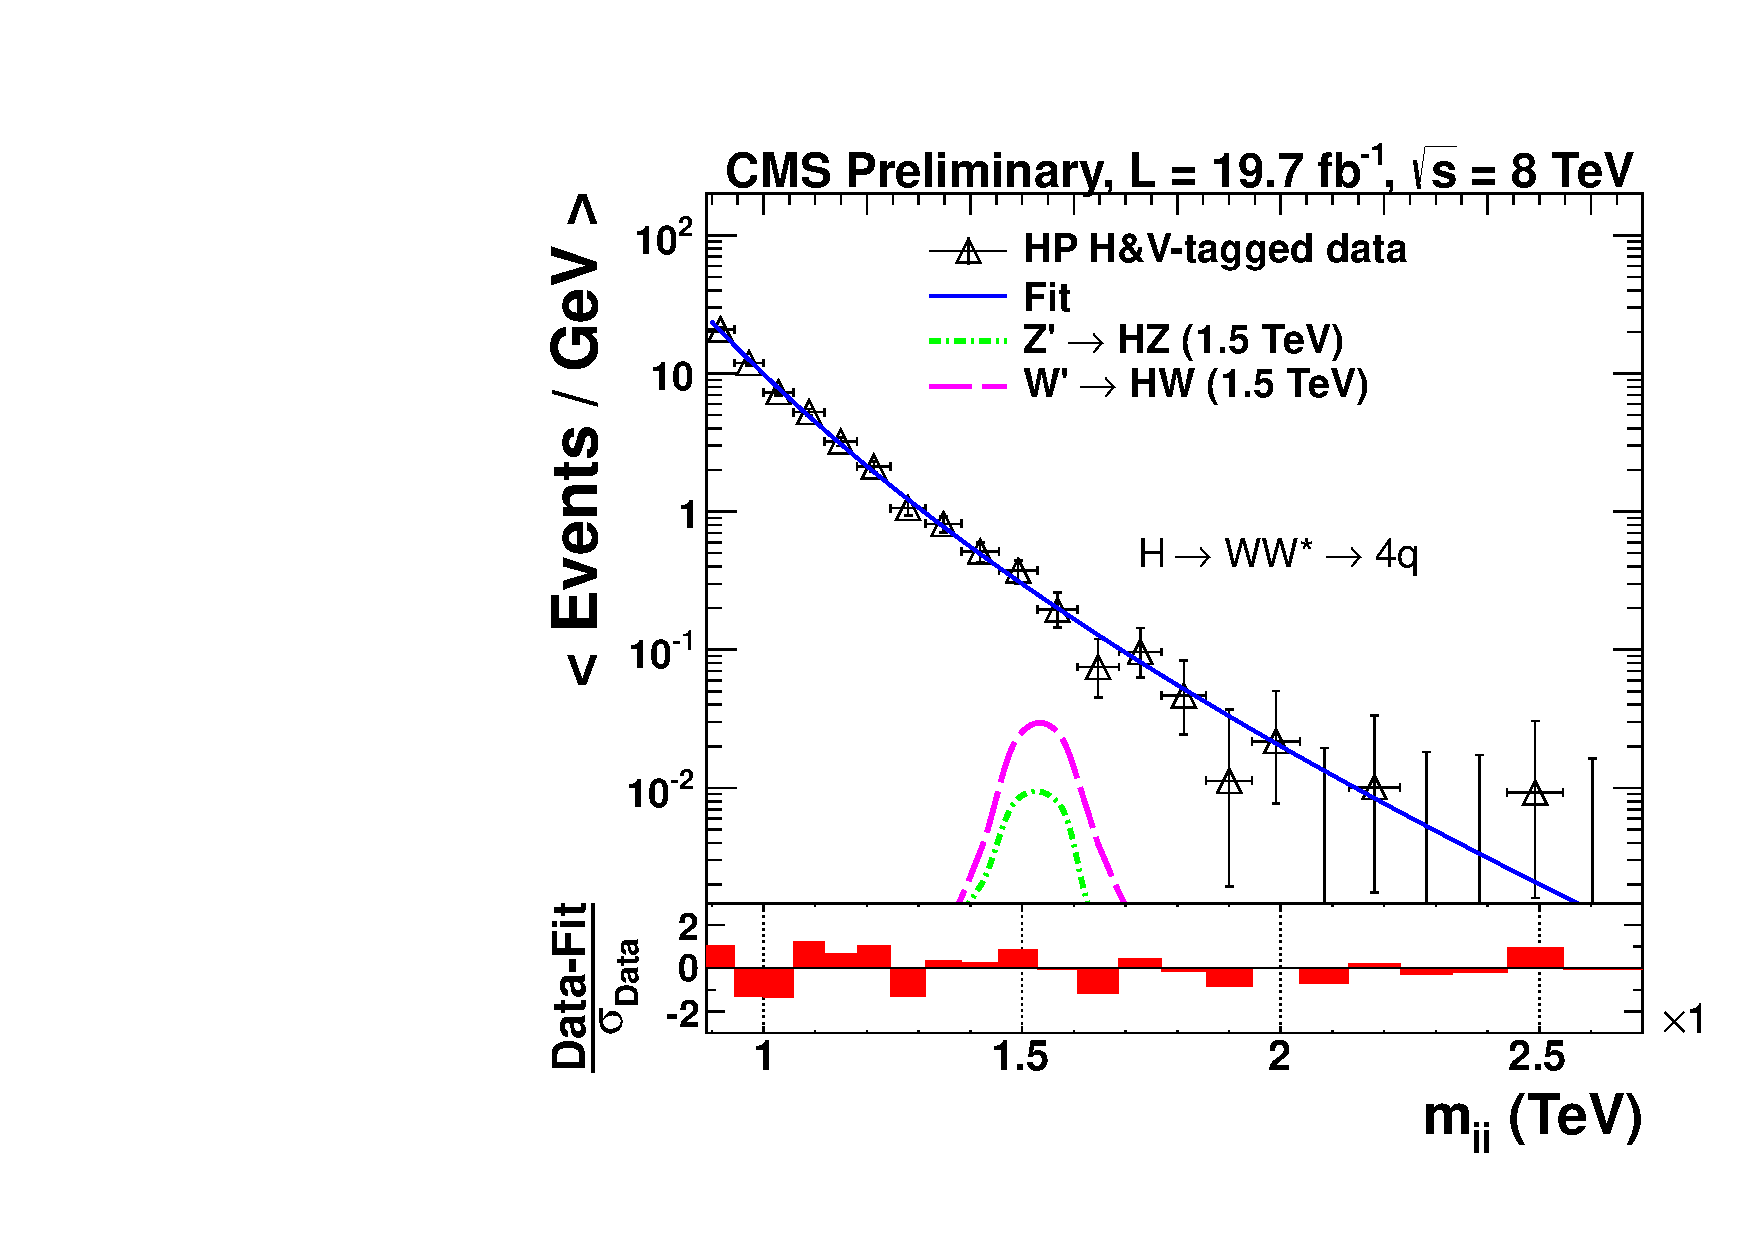
\includegraphics[width=0.51\textwidth]{EXO-14-009/HqqqqZqqfigs/FITS/HwwVqqFitAndPullHighP.pdf}
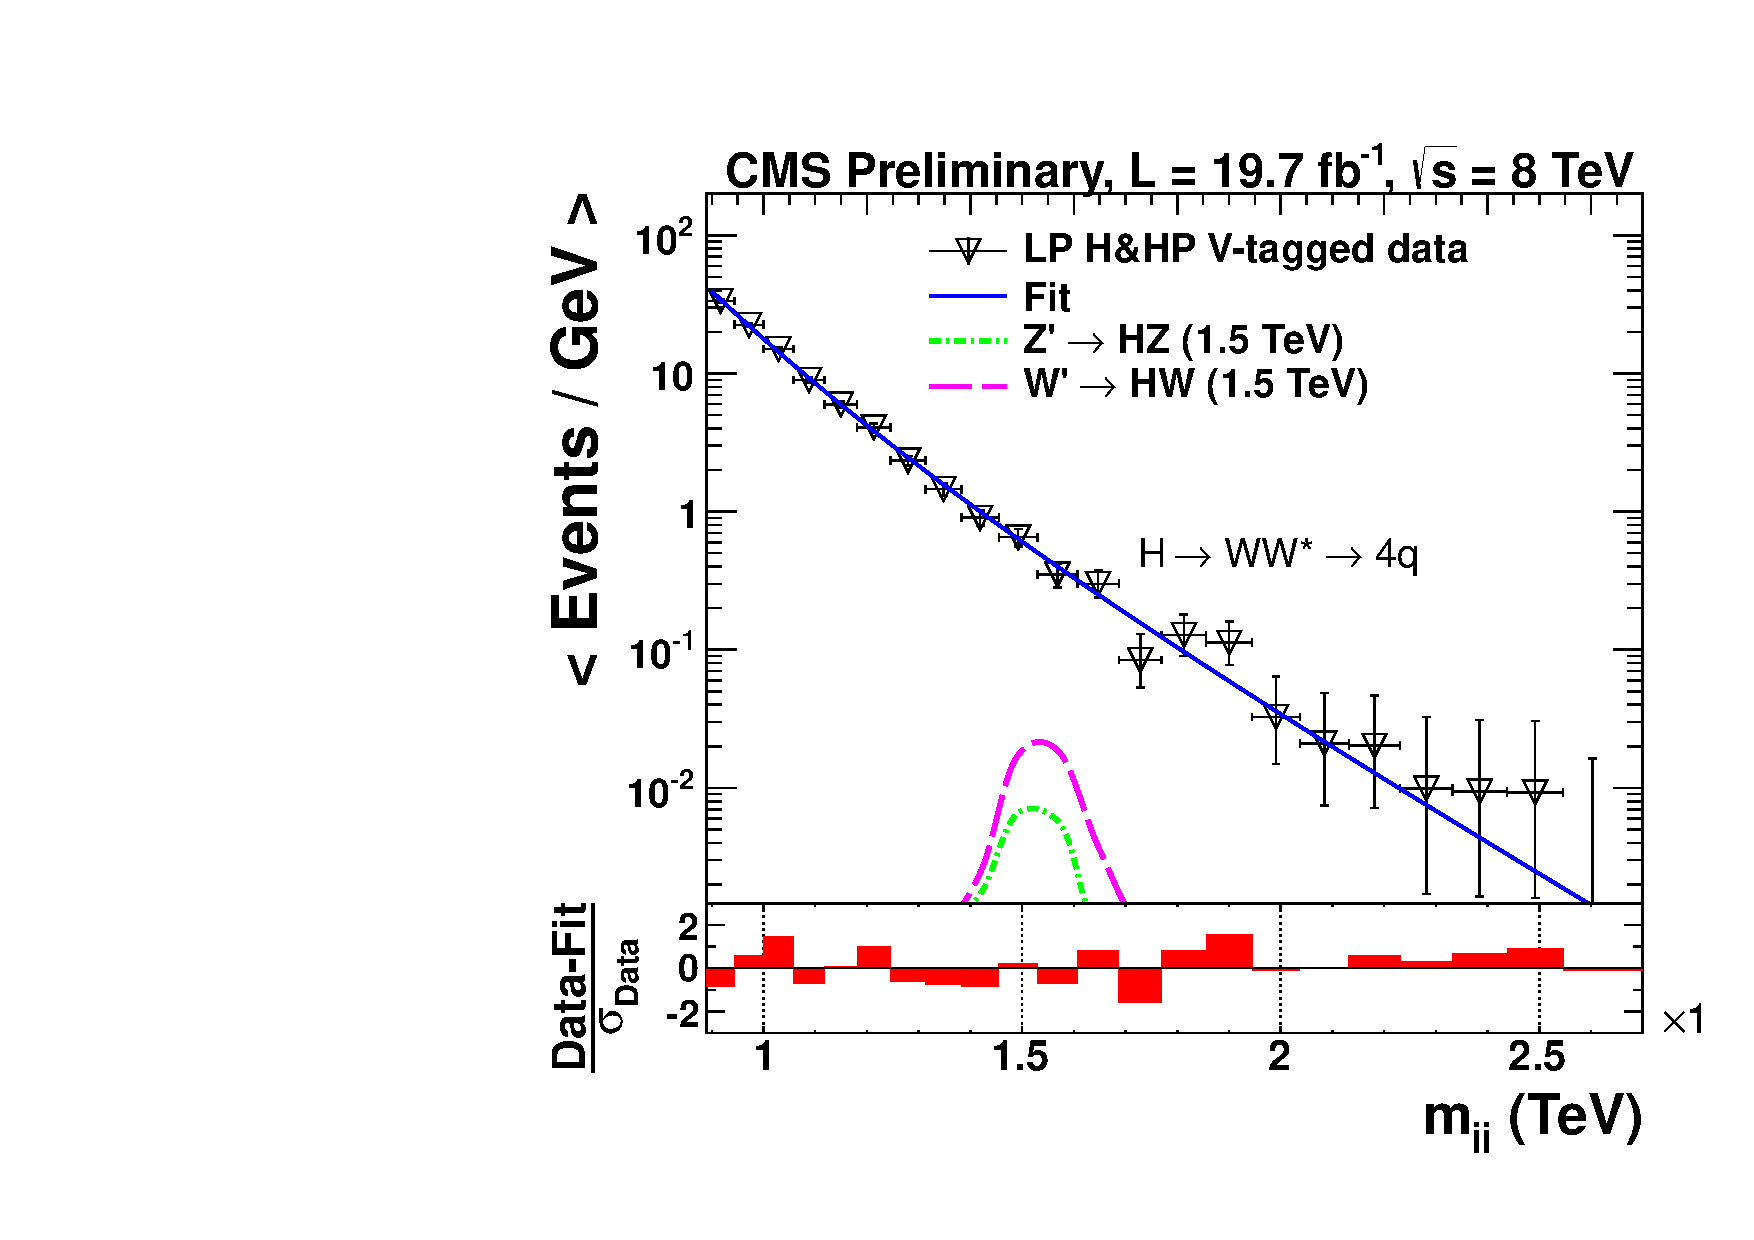
\includegraphics[width=0.49\textwidth]{EXO-14-009/HqqqqZqqfigs/FITS/HwwVqqFitAndPullLowH.pdf}
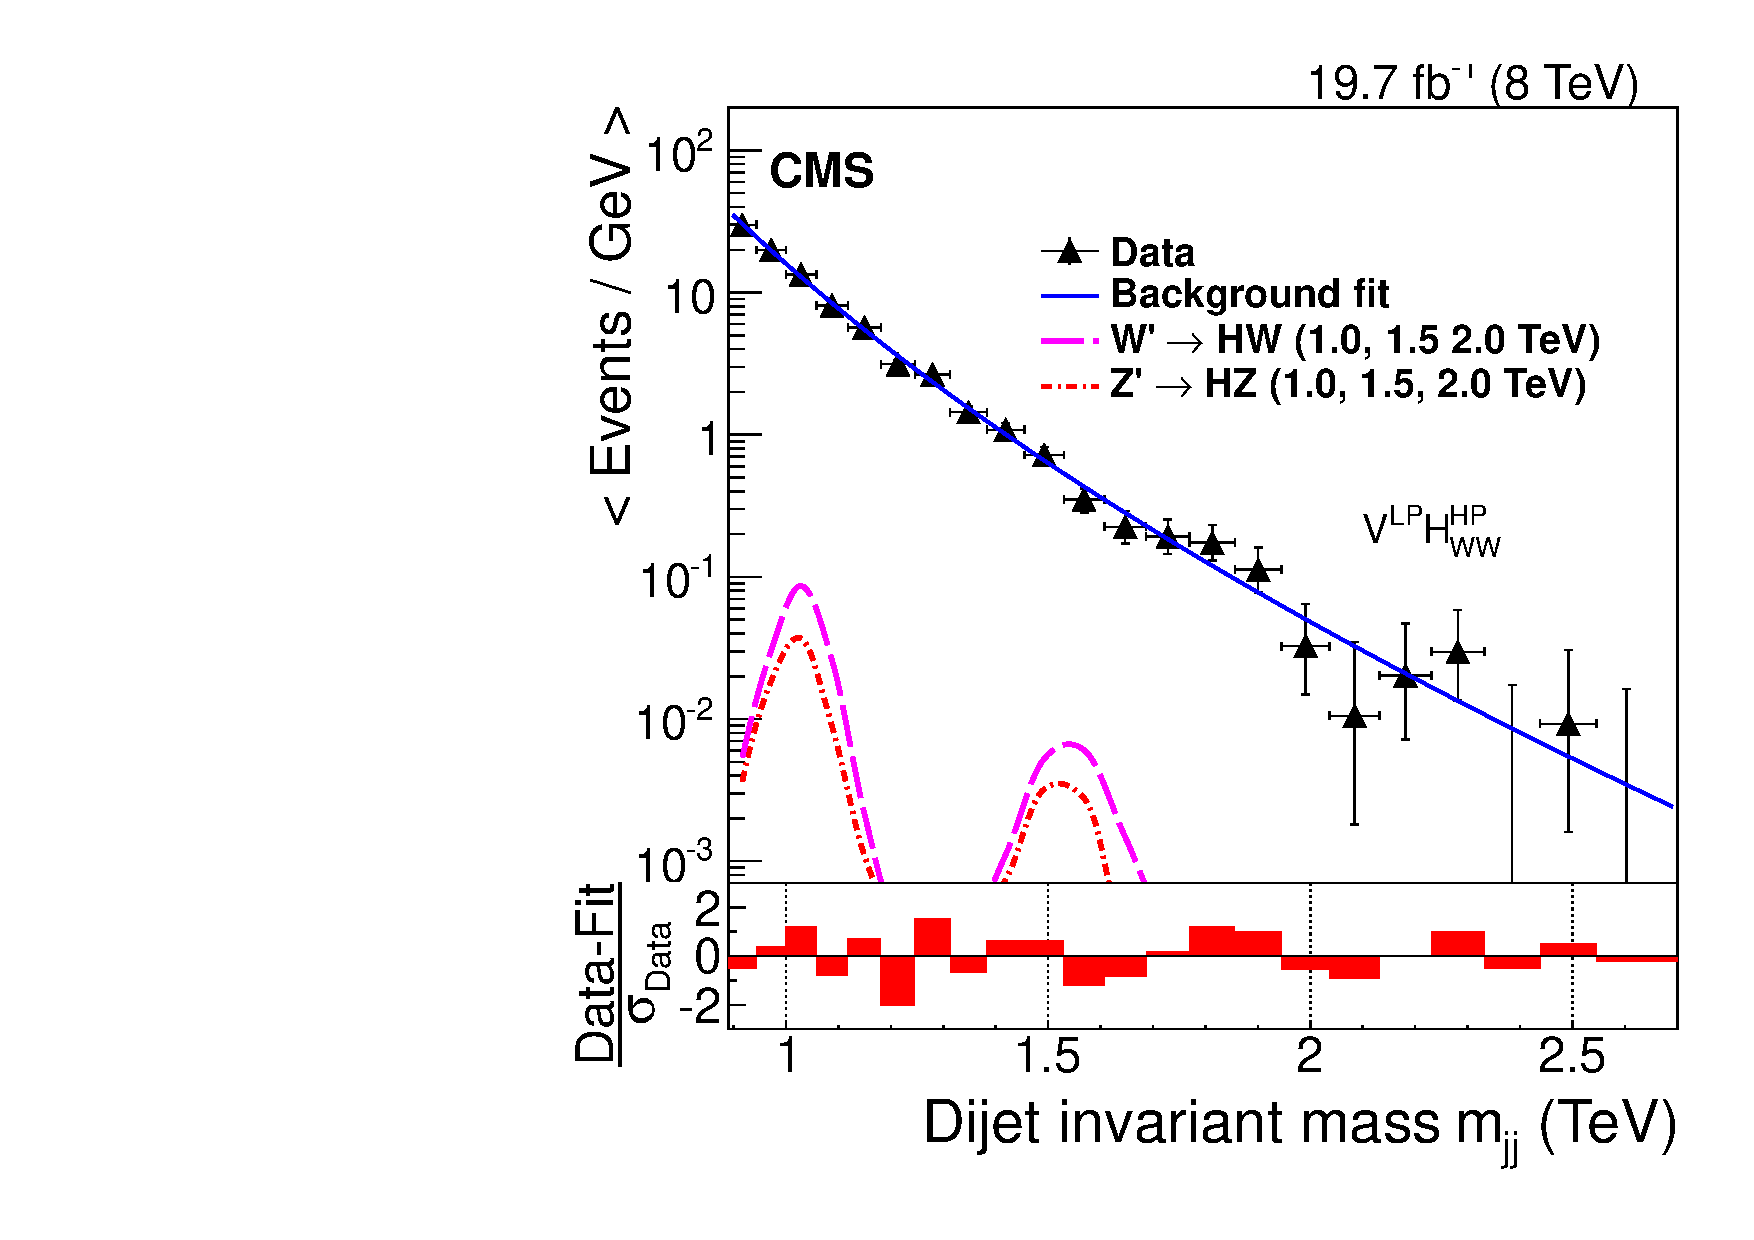
\includegraphics[width=0.49\textwidth]{EXO-14-009/HqqqqZqqfigs/FITS/HwwVqqFitAndPullLowV.pdf}
\end{center}
\caption{
Distributions in $m_\mathrm{jj}$ are shown for
   \HWWHP\ (top), \HWWLPH\ (bottom left), and 
   \HWWLPV\ (bottom right).  
    The solid curves represent the
   results of fitting Eq.~(\ref{eqParam}) to the data. The
   distributions for \HwwVqq 
   contributions, scaled to their corresponding cross sections, are
   given by the dashed and dash-dotted curves. 
   The vertical axis displays the number of events per bin, divided
   by the bin width.
Horizontal bars
through the data points indicate the bin width. 
The corresponding pull
   distributions
   $\frac{\text{Data}-\text{Fit}}{\sigma_{\text{Data}}}$, where
   $\sigma_{\text{Data}}$ represents the statistical uncertainty in
   the data in a bin in $m_\mathrm{jj}$, are shown below each
   $m_\mathrm{jj}$ plot. }
\label{fig:HwwZqqBG}
\end{figure}




\clearpage

